\section{Analytical quantities} 



To understand the dynamical properties of the BDC process, there are a handful of quantities for the focus of analysis.  



\subsection*{ ${I(t)}$, the non-catastrophe probability}

\vspace{3pt}
{\Large$$ I(t) = \pr{\xt \neq H|\; \xx_0 = 1}$$
$$\text{ \& }$$
$$\hat I(t) = \pr{\xt \notin \{0, H \}|\; \xx_0 = 1}$$}

\noindent
Given that the rupture state, $H$ is accessible from every non-zero state of the Markov process, eventual catastrophe is inevitable provided the process doesn't fixate by depletion to 0. Hence, either death or catastrophe is sure to happen at late time. $I(t)$ is the probability that the process has not experienced catastrophe prior to time $t$. 

 {\large $$I(t) = \frac{a(1-b) - b(1-a) \ee^{\lambda(a - b)t}}{(1-b) - (1-a) \ee^{\lambda(a - b)t}},$$}
 where 
$$a = \eta+\sqrt{\eta^2-\frac{\mu}{\lambda}}  \qquad  \text{ and } \qquad b =  \eta-\sqrt{\eta^2-\frac{\mu}{\lambda}},$$
with 
$$\eta = \frac{\lambda + \mu + \delta}{2\lambda}$$
This is the solution to a differential equation seen below. When $\mu>0$ and process death is possible.   It will tend down to the positive constant value, $b$, the likelihood of eventual  process death,
 $$\lrb{\lim_{t\to \infty}I(t) = \frac{-b(1-a)}{-(1-a)} = b}$$




\begin{figure}[H]
\xdef\mydelt{0.05}
\xdef\mybeta{1}
\xdef\mymu{0.2}
\begin{center}
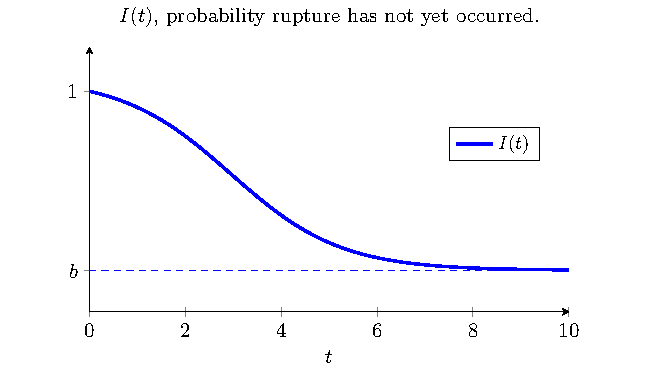
\includegraphics[width = 0.65\textwidth]{figures/IMG_ch4/I_of_t_1.pdf}
\end{center}
\caption{$I(t)$ plotted against time. Converges to $I_-$, representing the probability of eventual compartment recovery --- the birth death process dies out before rupture. $\beta=\mybeta$, $\mu=\mymu$, $\delta=\mydelt$}
\end{figure}



We can also consider the non-fixation probability, $\hat I(t)$, signifying the likelihood that at time $t$ the process has neither died, nor experienced catastrophe,
$$\hat I(t) = \pr{\xt \notin \{0, H \}|\; \xx_0 = 1}.$$ 
This will decline asymptotically to 0 signifying the eventual certainty of fixation one way or the other.  The solution is 

$$\hat I(t)  = \frac{2\eta}{1 - (1-2\eta)\ee^{2\eta\lambda t}},$$

$$\lim_{t\to \infty} \hat I(t) = 0.$$
The formulas for both $I(t)$ and $\hat I(t)$ are shown to result from their associated ODEs in the following section. Their form was first established by Kalin and Tavare in the 80s \cite{karlin1982linear}.



\begin{figure}[H]
\xdef\mydelt{0.05}
\xdef\mybeta{1}
\xdef\mymu{0.2}
\begin{center}
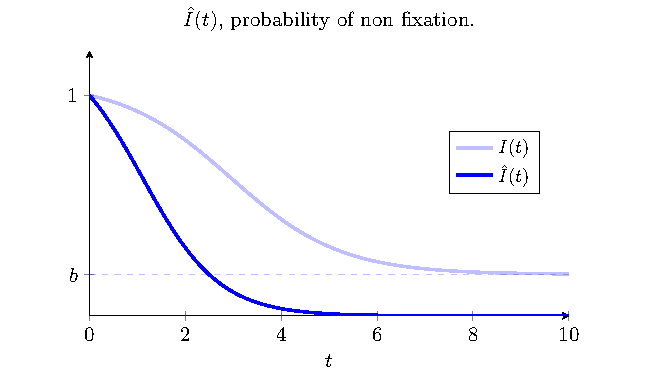
\includegraphics[width = 0.65\textwidth]{figures/IMG_ch4/I_of_t_2.pdf}
\end{center}
\caption{$\hat I(t)$ plotted against time. $\beta=\mybeta$, $\mu=\mymu$, $\delta=\mydelt$}
\end{figure}

\noindent
Suppose the process  begins with $k$ initial particles, $\xx_0 = k$. Each replicative unit gives rise to its own set of descendants, all behaving independently from one another. The likelihood through time that any one of those $k$ families will \textit{not} have led to catastrophe is $I(t)$. So it follows naturally, the probability that none of the $k$ families has led to the mass emigration is $\lrbs{I(t)}^k$;
$$  I_k(t) = \pr{\xt \neq H|\; \xx_0 = k} = \lrbs{I(t)}^k.$$
Likewise, when considering fixation more generally, 
$$\hat I_k(t) = \pr{\xt \notin \{0, H \}|\; \xx_0 = k}= \lrbs{\hat I(t)}^k.$$ 
(Is this correct?)



\subsection*{$J(t)$, replicative unit mean}

\vspace{3pt}
{\Large$$J(t) = \mean{\xt|\xx_0 = 1}$$}

\noindent
A given realisation of the process will rise and fall stochastically in steps for some time before ending up stuck either at 0 or, after catastrophe, at $H$. Following each of these fixation outcomes, the contribution of $\xt$ to the mean $J(t)$ is 0. So, supposing we observe 100 realisations, if at time $t=20$ all of them have have either died or undergone catastrophe, their sample mean would be 0 ($J_{\text{sample}}(20) = 0$).


From the initial condition, $\xx_0 = 1$, the process mean will go on to rise with realisations tending to increase, then fall as the likelihood of fixation grows asymptotically certain.

\begin{figure}[H]
\xdef\mydelt{0.05}
\xdef\mybeta{1}
\xdef\mymu{0.2}
\begin{center}
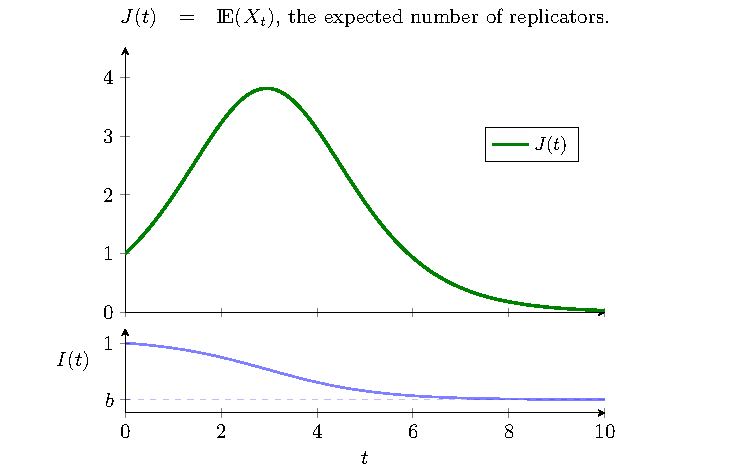
\includegraphics[width = 0.7\textwidth]{figures/IMG_ch4/J_of_t_1.pdf}
\end{center}
\caption{$J(t)$ plotted against time. $\beta=\mybeta$, $\mu=\mymu$, $\delta=\mydelt$}
\end{figure}

\noindent
It is given by the formula,

{\large$$J(t) = -\frac{\lambda(1-a)(1-b)(a-b)^2\ee^{\beta(a-b)t}}{\delta\big((1-b) - (1-a)\ee^{\lambda(a-b)t}\big)^2},$$}
which is obtained simply by differentiating $I(t)$ then multiplying by $-\delta^{-1}$. This follows from the equation $I' = -\delta J$ covered in more detail below.



\subsection*{$V(t)$, number of released units}

\vspace{3pt}
{\Large$$V(t) = \mean{\wt| \xx_0 = 1}$$}

\noindent
Over time, the process will either decline to 0, or transition to the catastrophe state, $H$. In which case, $\wt$ will be set at a geometrically distributed quantity seen in the final numeric value of $\xt$. $V(t)$, the expected post rupture count, incorporates all situations, whether $\wt$ is zero or not:

{\large $$V(t) = \frac{(\lambda - \mu)}{\delta}\big[1-I(t)\big] -J(t)+1. $$}
At late time, realisations which ended in both catastrophe, and death will constitute the value of $\lim_{t\to\infty} V(t) = V_{\infty}$.

$$V_{\infty} = \frac{(\lambda - \mu)}{\delta}\big[1-b\big]+1,$$
as $I\to b$ and $J \to 0$; when $\mu = 0$, 
$$V_{\infty} = \frac{\lambda }{\delta}+1.$$

For the case where death is included ($\mu>0$), the formula, $V_{\infty}$, takes into account eventualities in which the process did not attain catastrophe.
We may also extract the mean burst size proper by conditioning for cases which did experienced rupture, effectively discounting the dead realisations. This is done by dividing $V(t)$ by the likelihood of process catastrophe, $1-I(t)$. This is taken from the basic logic,
$$\mean{\wt} = \cancelto{0}{\mean{\wt | \text{no rupture}} I(t) }  + \mean{\wt | \text{rupture}} (1 - I(t)) $$
$$ \mean{\wt | \text{rupture}}  =  \frac{\mean{\wt}}{1 - I(t)},$$
$$\frac{V(t)}{1 - I(t)} $$
represents the expected burst size given catastrophe has taken place by time $t$. The ``overall'' burst size mean is seen in the late time value of this, incorporating all process realisations which experience rupture regardless of when:

\begin{align*}
\mean{\mathcal{K}} = \lim_{t\to \infty} \frac{V(t)}{1 - I(t)} &=  \frac{V_{\infty}}{1 - b} \\
&= \frac{\lambda-\mu}{\delta} + \frac{1}{1-b},
\end{align*}
(recalling that $b$ is the probability of ultimate process death). Notice the alignment $\mean{\mathcal{K}} = V_\infty$ when $\mu=0$. 



PLOT $\mean{\mathcal{K}}$ against $\delta$ for $\mu = 0$, $\lambda = 1$


	
\begin{figure}[H]
\begin{center}

\xdef\mydelt{0.05}
\xdef\mybeta{1}
\xdef\mysum{0.151}
\xdef\mymu{0.2}


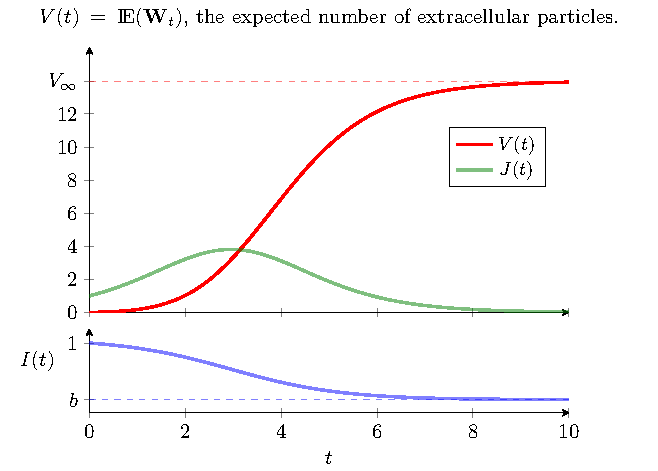
\includegraphics[width = 0.7\textwidth]{figures/IMG_ch4/V_of_t_1.pdf}

\end{center}
\caption{$V(t)$ plotted against time. $\beta=\mybeta$, $\mu=\mymu$, $\delta=\mydelt$.}
\end{figure}



\subsection*{$K(t)$, second moment of $\xt$}

\vspace{3pt}
{\Large$$K(t) = \mean{\xt^2| \xx_0 = 1}$$}

\noindent
We became interested in this quantity because it showed up in a term of the ODE describing change in $J(t)$:
$$\ddt{J} = (\lambda - \mu) J - \delta \mean{\xt^2}.$$
This final term results from the following reasoning. With rate $\delta \xt$, the value of $J(t)$ is reduced by $\xt$. So the expected deduction to $\xt$ by catastrophe over an infinitesimal duration is $\mean{ -\delta \xt^2 \delt}$. Hence, in deriving the above ODE, we find the contribution $-\delta \mean{\xt^2}$.



%%%%%%%%%%%%%%%%%%%%%%%%%%%%%%%%%%%%%%%%%%%%%%%%%%%%%%%%%%%%%%%%%%%%%%%%%%%%%%%%%%%%%%%%%%%%%%%%%%%%%%%%%%%
